% 12pt: grandezza carattere
% a4paper: formato a4
% openright: apre i capitoli a destra
% twoside: serve per fare un
% documento fronteretro
% report: stile tesi (oppure book)
\documentclass[12pt,a4paper,openright,twoside]{report}

%libreria per scrivere in italiano
\usepackage[italian]{babel}

% libreria per accettare i caratteri
% digitati da tastiera come ?
% si può usare anche
% \usepackage[T1]{fontenc}
% però con questa libreria
% il tempo di compilazione
% aumenta
\usepackage[latin1]{inputenc}

% libreria per impostare il documento
\usepackage{fancyhdr}

% libreria per avere l'indentazione all'inizio dei capitoli, ...
\usepackage{indentfirst}

%libreria per mostrare le etichette
%\usepackage{showkeys}

% libreria per inserire grafici
\usepackage{graphicx}

% libreria per utilizzare font particolari ad esempio \textsc{}
\usepackage{newlfont}

% librerie matematiche
\usepackage{amssymb}
\usepackage{amsmath}
\usepackage{latexsym}
\usepackage{amsthm}

% librerie per mostrare il codice sorgente
\usepackage{listings, xcolor}
\renewcommand{\lstlistingname}{Codice sorgente}
\renewcommand{\lstlistlistingname}{Codici sorgenti}
% impostano i margini
\oddsidemargin=30pt
\evensidemargin=20pt

% serve per la sillabazione: tra parentesi vanno inserite come nell'esempio le parole
% che latex non riesce a tagliare nel modo giusto andando a capo.
\hyphenation{sil-la-ba-zio-ne pa-ren-te-si}

% comandi per l'impostazione della pagina, vedi il manuale della libreria fancyhdr per ulteriori delucidazioni
\pagestyle{fancy}\addtolength{\headwidth}{20pt}
\renewcommand{\chaptermark}[1]{\markboth{\thechapter.\ #1}{}}
\renewcommand{\sectionmark}[1]{\markright{\thesection \ #1}{}}
\rhead[\fancyplain{}{\bfseries\leftmark}]{\fancyplain{}{\bfseries\thepage}}
\cfoot{}

%comando per impostare l'interlinea
\linespread{1.3}

\begin{document}

\begin{titlepage}
% crea un ambiente libero da vincoli di margini e grandezza caratteri: si pu\`o modificare
% quello che si vuole, tanto fuori da questo ambiente tutto viene ristabilito

% elimina il numero della pagina
\thispagestyle{empty}

% imposta il margina superiore a 6.5cm
\topmargin=6.5cm

% incolonna la scrittura a destra
\raggedleft

% aumenta la grandezza del carattere a 14pt
\large

% emfatizza (corsivo) il carattere
\em

%\ldots lascia tre puntini
%\ldots

% va in una pagina nuova
\newpage

% non numera l'ultima pagina sinistra
\clearpage{\pagestyle{empty}\cleardoublepage}
\end{titlepage}

\pagenumbering{roman} % serve per mettere i numeri romani
\chapter*{Introduzione} % crea l'introduzione (un capitolo non numerato)

% imposta l'intestazione di pagina
\rhead[\fancyplain{}{\bfseries INTRODUZIONE}]{\fancyplain{}{\bfseries\thepage}}
\lhead[\fancyplain{}{\bfseries\thepage}]{\fancyplain{}{\bfseries INTRODUZIONE}}

% aggiunge la voce Introduzione nell'indice
\addcontentsline{toc}{chapter}{Introduzione}
% \ldots
Questo lavoro ha l'obiettivo di implementare sul simulatore Alchemist il modello ad agenti.

Alchemist \`e un meta-simulatore estendibile, ispirato alla chimica stocastica e adatto al calcolo pervasivo e ai sistemi distribuiti. Fornisce un meta-modello flessibile, sul quale gli sviluppatori legano le proprie astrazioni, realizzando una 'incarnazione'.

Il modello ad agenti a cui si fa riferimento \`e quello BDI (Beliefs, Desires, Intentions) che \`e ispirato al modello del comportamento umano.


% non numera l'ultima pagina sinistra
\clearpage{\pagestyle{empty}\cleardoublepage}

%crea l'indice
\tableofcontents

% imposta l'intestazione di pagina
\rhead[\fancyplain{}{\bfseries\leftmark}]{\fancyplain{}{\bfseries\thepage}}
\lhead[\fancyplain{}{\bfseries\thepage}]{\fancyplain{}{\bfseries INDICE}}

% non numera l'ultima pagina sinistra
\clearpage{\pagestyle{empty}\cleardoublepage}

% crea l'elenco delle figure
\listoffigures

% non numera l'ultima pagina sinistra
\clearpage{\pagestyle{empty}\cleardoublepage}

% crea l'elenco delle tabelle
%\listoftables

% non numera l'ultima pagina sinistra
\clearpage{\pagestyle{empty}\cleardoublepage}

%% % crea l'elenco dei codici sorgenti
 \lstlistoflistings
%%
%% % non numera l'ultima pagina sinistra
%% \clearpage{\pagestyle{empty}\cleardoublepage}

%-%-%-%-%-%-%-%-%-%-%-%-%-%-%-%-%-%-%-%-%-%-%-%-%-%-%-%-%-%-%-%-%-%-%-%-%-%-%-%-
\chapter{Alchemist}
% imposta l'intestazione di pagina
\lhead[\fancyplain{}{\bfseries\thepage}]{\fancyplain{}{\bfseries\rightmark}}
% mette i numeri arabi
\pagenumbering{arabic}
Alchemist fornisce un ambiente di simulazione sul quale \`e possibile sviluppare nuove incarnazioni, ovvero nuove definizioni di modelli sviluppati su di esso.

%++-++-++-++-++-++-++-++-++-++-++-++-++-++-++-++-++-++-++-++-++-++-++-++-++-++-
\section{Il meta-modello}
Il meta-modello di Alchemist pu\`o essere compreso con la figura \ref{fig:alchemistModel}.
%crea l'ambiente figura;
\begin{figure}[h] % [h] sta per here, cioè la figura va qui
\begin{center} % centra nel mezzo della pagina la figura
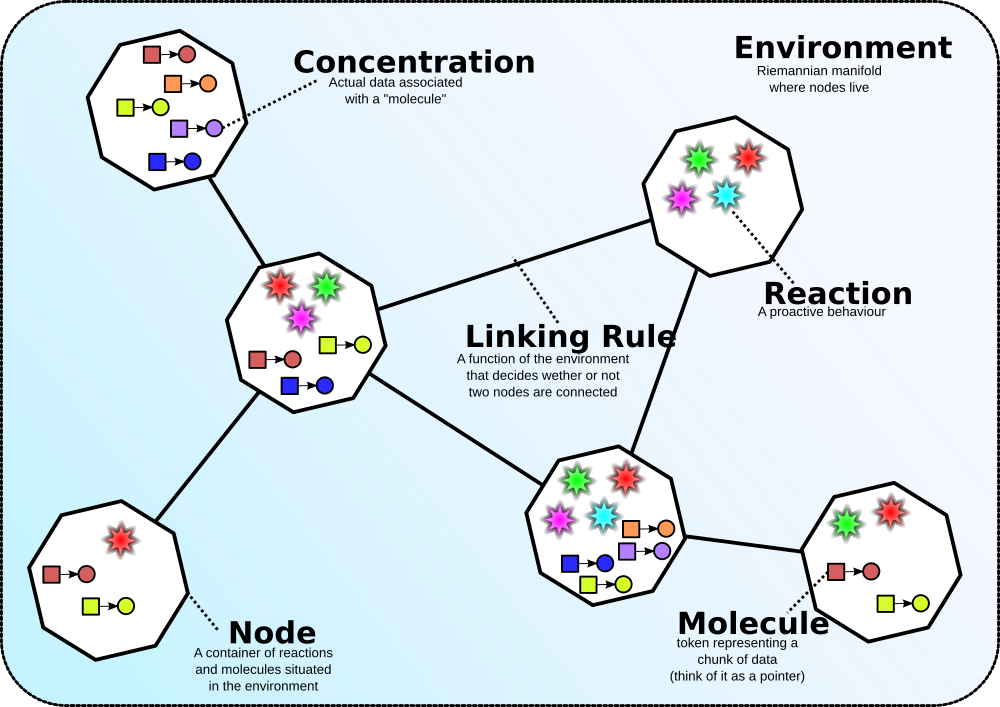
\includegraphics[width=12.5cm]{images/model.png} % inserisce una figura larga 12.5cm
% inserisce la legenda ed etichetta la figura con \label{fig:prima}
\caption[Illustrazione meta-modello di Alchemist]{Illustrazione meta-modello di Alchemist} \label{fig:alchemistModel}
\end{center}
\end{figure}

L'\textbf{\textit{Environment}} \`e l'astrazione dello spazio ed \`e anche l'entit\`a pi\`u esterna che funge da contenitore per i nodi. Conosce la posizione di ogni nodo nello spazio ed \`e quindi in grado di fornire la distanza tra due di essi e ne permette inoltre lo spostamento.

\`E detta \textbf{\textit{Linking rule}} una funzione dello stato corrente dell'environemnt che associa ad ogni nodo un \textbf{\textit{Vicinato}}, il quale \`e un entit\`a composta da un nodo centrale e da un set di nodi vicini.

Un \textbf{\textit{Nodo}} \`e un contenitore di molecole e reazioni che \`e posizinato all'interno di un environment.

La \textbf{\textit{Molecola}} \`e il nome di un dato, paragonabile a quello che rappresenta il nome di una variabile per i linguaggi imperativi.
Il valore da associare ad una molecola \`e detto \textbf{\textit{Concentrazione}}.

%crea l'ambiente figura;
\begin{figure}[h] % [h] sta per here, cioè la figura va qui
\begin{center} % centra nel mezzo della pagina la figura
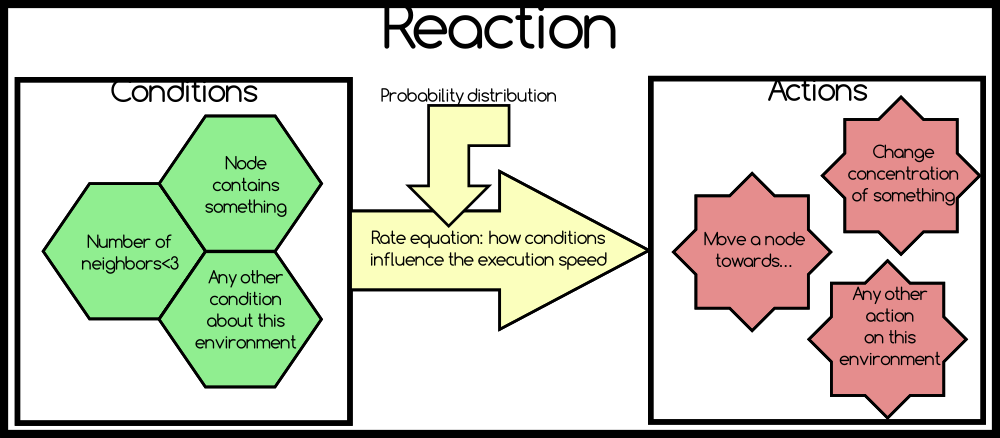
\includegraphics[width=14cm]{images/reaction.png} % inserisce una figura larga 12.5cm
% inserisce la legenda ed etichetta la figura con \label{fig:prima}
\caption[Illustrazione modello reazione di Alchemist]{Illustrazione modello reazione di Alchemist} \label{fig:alchemistReaction}
\end{center}
\end{figure}

Una \textbf{\textit{Reazione}} \`e un qualsiasi evento che pu\`o cambiare lo stato dell'environment ed \`e. definita tramite una lista di condizioni, una o pi\`u azioni.
\\La frequenza con cui avvengono dipende da:
\begin{itemize}
\item un parametro statico di frequenza;
\item il valore di ogni condizione;
\item un'equazione di frequenza che combina il tasso statico e il valore delle condizioni restituendo la frequenza istantanea;
\item una distribuzione temporale.
\end{itemize}
Ogni nodo contiene un set di reazioni che pu\`o essere anche vuoto.

Per comprendere meglio il meccanismo di una reazione si pu\`o osservare la figura \ref{fig:alchemistReaction}.

Una \textbf{\textit{Condizione}} \`e una funzione che prende come input l'environment corrente e restituisce come output un booleano e un numero. Se la condizione non si verifica, le azioni associate a quella reazione non saranno eseguite. In relazione a parametri di configurazione e alla distribuzione temporale, una condizione potrebbe influire sulla velocit\`a della reazione.

La \textbf{\textit{Distribuzione temporale}} indica il numero di eventi che si verificano successivamente ed indipendentemente in un dato intervallo di tempo.

Un'\textbf{\textit{Azione}} \`e la definizione di una serie di operazioni che modellano un cambiamento nel nodo o nell'environment.

In Alchemist un'incarnazione \`e un'istanza concreta del meta-modello appena descritta e che implementa una serie di componenti base come: la definizione di una molecola e del tipo di dati della concentrazione, un set di condizioni, le azioni e le reazioni. Incarnazioni diverse possono modellare universi completamente differenti.

%++-++-++-++-++-++-++-++-++-++-++-++-++-++-++-++-++-++-++-++-++-++-++-++-++-++-
\section{Scrivere una simulazione}
% style for general source code
\lstset{
  numberstyle=\footnotesize\color{black},
  basicstyle=\ttfamily,
  breakatwhitespace=false,
  breaklines=true,
  captionpos=b,
  keepspaces=true,
  numbers=left,
  numbersep=0pt,
  showspaces=false,
  showstringspaces=false,
  showtabs=false,
  tabsize=2,
  frame=tb
  %label=incarnationYAML,
  %caption={First verbatim}
  %language=Java
}
Il linguaggio da utilizzare per scrivere le simulazioni in Alchemist \`e YAML e quello che il parser del simulatore si aspetta in input \`e una mappa YAML.
\\
Nei prossimi paragrafi verr\`a mostrato quali sezioni si possono inserire e come utilizzarle per creare la simulazione che si vuole realizzare.

La sezione \textbf{incarnation} \`e obbligatoria. Il parser YAML si aspetta una stringa che rappresenta il nome dell'incarnazione da utilizzare per la simulazione.
\medskip
\begin{lstlisting}[firstnumber=last,caption={Incarnazione}]
  incarnation: agent
\end{lstlisting}

Nelle prossime occorrenze, dove si utilizza la chiave 'type' il valore associato fa riferimento al nome di una classe. Se il nome passato non \`e completo, ovvero non \`e comprensivo del percorso fino alla classe, Alchemist provveder\`a a cercare la classe tra i packages.

Per dichiarare variabili che poi potranno essere richiamate all'interno del file di configurazione della simulazione si pu\`o procedere in questo modo.
\medskip
\begin{lstlisting}[firstnumber=last,caption={Variabili simulazione}]
  variables:
    myVar: &myVar
      par1: 0
      par2: "string"
    mySecondVar: &myVar2
      par: "value"
\end{lstlisting}

Con la keyword \textbf{environment} si pu\`o scegliere quale definizione di ambiente utilizzare per la simulazione.
\medskip
\begin{lstlisting}[firstnumber=last,caption={Environment}]
  environment:
    type: OSMEnvironment
    parameters: [/maps/foo.pbf]
\end{lstlisting}
Questo parametro \`e opzionale e di default \`e uno spazio continuo bidimensionale: ometterlo equivale a scrivere la seguente configurazione.
\medskip
\begin{lstlisting}[firstnumber=last,caption={Default environment}]
  environment:
    type: Continuous2DEnvironment
\end{lstlisting}


\textbf{POSITION}
\\
\textbf{TODO POSITION??}
\\
\\
I collegamenti tra i nodi che verranno utilizzati nella simulazione sono specificati nella sezione \textbf{network-model}. Un esempio per la costruzione di collegamenti \`e il seguente.
\medskip
\begin{lstlisting}[firstnumber=last,caption={Funzione linking-rule}]
  network-model:
    type: EuclideanDistance
    parameters: [10]
\end{lstlisting}
Anche questo \`e un parametro opzionale e di default non ci sono collegamenti, ovvero i nodi nell'environemnt non sono collegati, ed \`e descritto con il seguente formalismo.
\medskip
\begin{lstlisting}[firstnumber=last,caption={Default linking-rule}]
  network-model:
    type: NoLinks
\end{lstlisting}

Il posizionamento dei nodi viene gestito dalla sezione \textbf{displacements}. Questa sezione pu\`o contenere uno o pi\`u definizioni di disposizioni per i nodi.
Il parametro 'in' si definisce la geometria all'interno del quale verranno disposti i nodi, utilizzando ad esempio punti o figure come cerchi o rettangoli, mentre il parametro 'programs' definisce le reazioni da associare ad ogni nodo di quella certa disposizione.
\\
Esempi di classi utilizzabili nel parametro 'in' sono ad esempio Point e Circle.
La classe Circle necessata di quattro parametri da passare nel seguente ordine: il numero di nodi da disporre, la coordinata x del centro, la coordinata y del centro, il raggio del cerchio. Per la classe Point \`e sufficiente fornire in ordine la coordinata x e la coordinata y.

Il parametro 'programs' rappresenta le reazioni da associare ai nodi ed accetta una lista di reazioni le quali a loro volta sono formate da una lista di parametri. Un'esempio di definizione di una reazione \`e utilizzando 'time-distribution' (valore utilizzato per settare la freqeunza) e 'program' (parametro che viene ricevuto alla creazione della reazione e che pu\`o essere passato per instanziare condizioni e azioni).
Un'esempio di displacements \`e il seguente.
\medskip
\begin{lstlisting}[firstnumber=last,caption={Disposizione nodi e reazioni associate}]
  displacements:
    - in: {type: Circle, parameters: [5,0,0,2]}
      programs:
      -
        - time-distribution: 1
          program: "reactionParam"
        - time-distribution: 2
          program: "doSomethingParam"
    - in: {type: Point, parameters: [1,1]}
      programs:
      -
        - time-distribution: 1
          program: "pointReactionParam"
\end{lstlisting}


%-%-%-%-%-%-%-%-%-%-%-%-%-%-%-%-%-%-%-%-%-%-%-%-%-%-%-%-%-%-%-%-%-%-%-%-%-%-%-%-
\chapter{Agenti}
% imposta l'intestazione di pagina
\lhead[\fancyplain{}{\bfseries\thepage}]{\fancyplain{}{\bfseries\rightmark}}

Un'agente \`e un entit\`a che agisce in modo autonomo e continuo in uno spazio condiviso con altri agenti. Le caratteristiche principali di un agente sono: autonomia, proattivit\`a e reattivit\`a. Gli agenti sono formati da un nome, che \`e una caratteristica statica, e da componenti dinamici come lo stato.

%++-++-++-++-++-++-++-++-++-++-++-++-++-++-++-++-++-++-++-++-++-++-++-++-++-++-
\section{Agenti BDI}
Gli agenti BDI forniscono un meccanismo per separare le attivit\`a di selezione di un piano fra quelli presenti nella sua teoria dall'esecuzione del piano attivo, permettendo di bilanciare il tempo speso nella scelta del piano e quello per eseguirlo.

I \textbf{\textit{Beliefs}} sono informazioni dello stato dell'agente, ovvero ci\`o che l'agente sa del mondo (di se stesso e degli altri agenti), e possono comprendere regole di inferenza per permettere l'aggiunta di nuovi beliefs. L'insieme dei belief di un agente \`e detto 'belief base' o 'belief set' e si pu\`o modificare nel tempo.

I \textbf{\textit{Desires}} sono tutti i possibili piani che l'agente potrebbe eseguire. Rappresentano gli obiettivi o le situazioni che l'agente vorrebbe realizzare o portare a termine. I \textbf{goals} sono desires che l'agente persegue attivamente: per questo motivo, in generale, i piani desiderabili possono non essere coerenti tra loro mentre i goals \`e bene che lo siano.

I \textbf{\textit{Intentions}} sono piani a cui l'agente ha deciso di lavorare o a cui sta gi\`a lavorando. I piani sono sequenze di azioni che un agente pu\`o eseguire per raggiungere una intention. I piani possono contenerne altri al loro interno.

Gli \textbf{\textit{Eventi}} innescano le attivit\`a reattive degli agenti il cui risultato pu\`o essere l'aggiornamento dei beliefs, la chiamata ad altri piani o la modifica di goals.

Il ciclo di ragionamento di un agente avviene come descritto in figura \ref{fig:reasoningCicle}.
%crea l'ambiente figura;
\begin{figure}[h] % [h] sta per here, cioè la figura va qui
\begin{center} % centra nel mezzo della pagina la figura
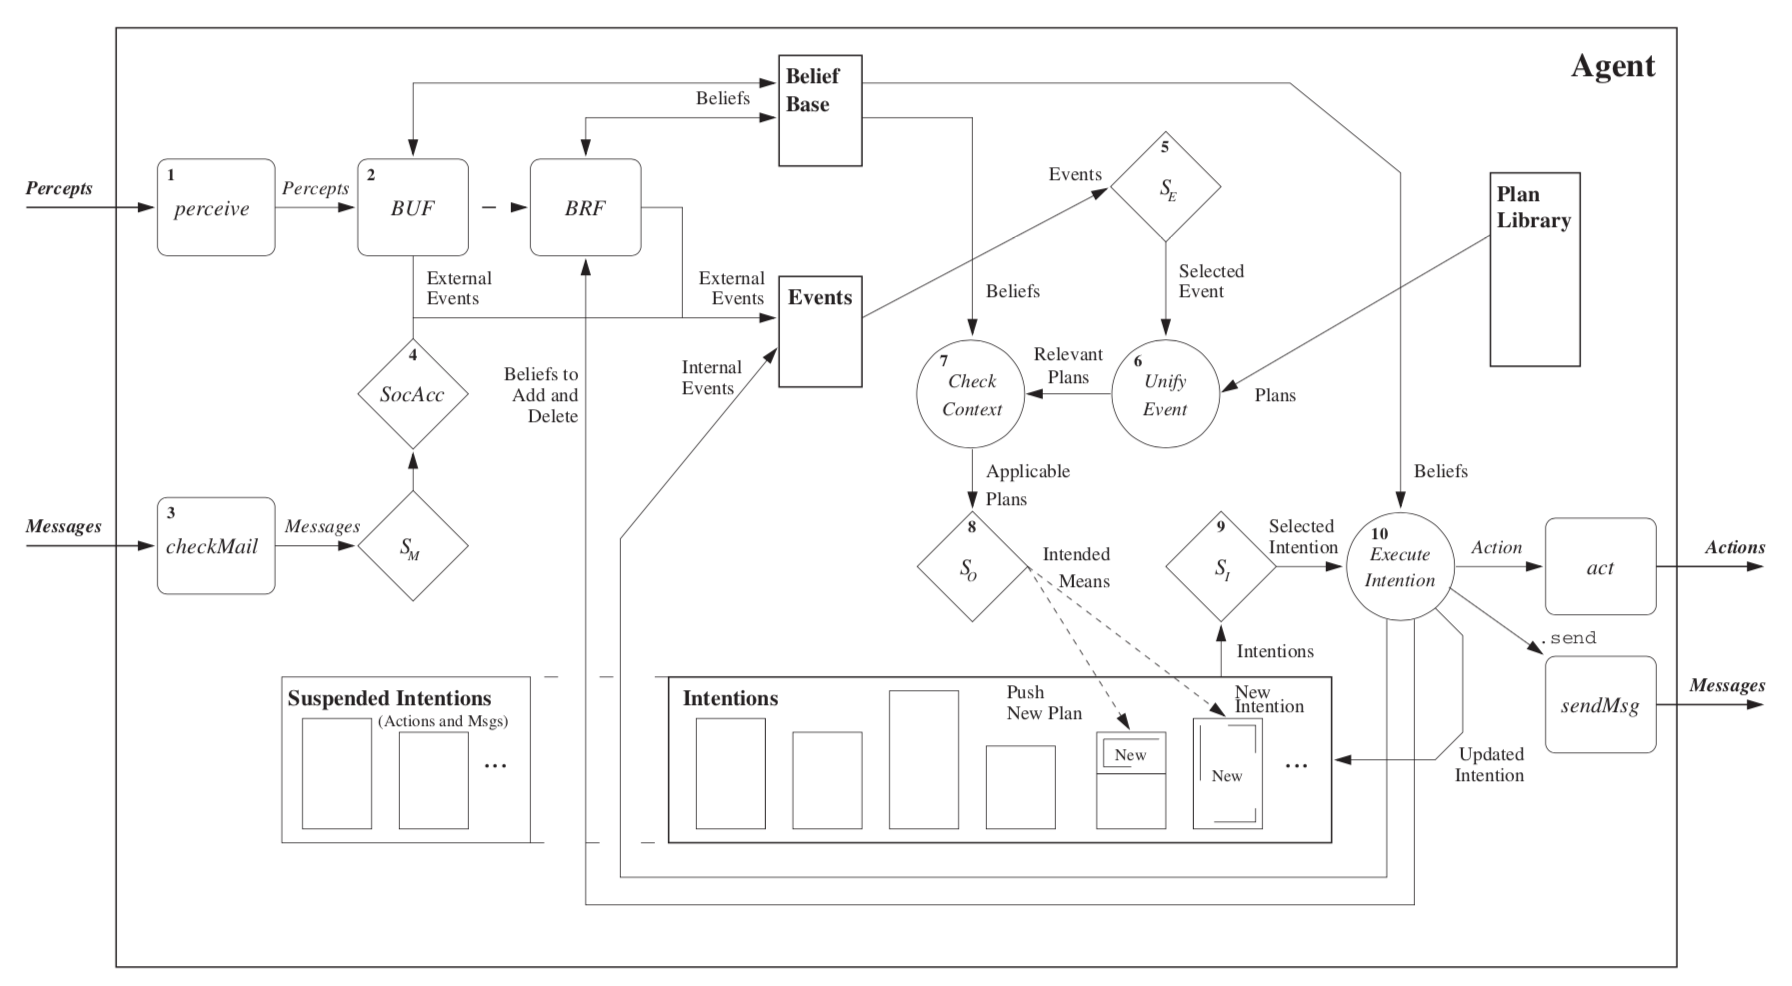
\includegraphics[width=16cm]{images/reasoningCicle.png} % inserisce una figura larga 12.5cm
% inserisce la legenda ed etichetta la figura con \label{fig:prima}
\caption[Ciclo di ragionamento di un agente]{Ciclo di ragionamento di un agente} \label{fig:reasoningCicle}
\end{center}
\end{figure}

%++-++-++-++-++-++-++-++-++-++-++-++-++-++-++-++-++-++-++-++-++-++-++-++-++-++-
\section{Ciclo di ragionamento}
RIVEDERE IL PEZZO QUI SOTTO E CONTINUARLO....
\\
\\
\\
La prima cosa che fa un agente nel ciclo di ragionamento \`e controllare l'ambiente per aggiornare i \textit{beliefs} con lo stato attuale. Quindi \`e necessario che l'agente abbia dei componenti per percepire i cambiamenti dell'ambiente. Una volta ottenuta la lista dei cambiamenti percepiti \`e necessario aggiornare la \textit{belief base} (che contiene l'insieme dei \textit{beliefs} dell'utente allo stato attuale).
\\
\\
// \textbf{TODO CONTINUARE} la descrizione del ciclo di ragionamento dell'agente....
% Modello ad agenti (JASON)
% Il funzionamento di un agente (reasoning cicle) prevede le seguenti fasi:
% - percezione di un cambiamento nell’environment e aggiornamento dei belief in base ai percepts ottenuti
% - ricezione di messaggi da parte di altri agenti e selezione dei messaggi accettabili
% - selezione di un evento tra quelli presenti nel set di quelli pending tramite politica FIFO
% - scelta dei piani rilevanti (dal set di piani della libreria) in base all’evento corrente e, quindi, selezione (dal set di piani rilevanti) di quelli applicabili in base al contesto dell’agente
% - selezione di un piano che verrà inserito nel set di intention dell’agente
% - selezione e esecuzione dell’intention da eseguire
% - se vi sono risposte disponibili, l’interprete inserisce le intention rilevanti nel set per permetterne la scelta nel prossimo ciclo
%
% Ad ogni ciclo vengono presi solamente un percept/messaggio, scelto un singolo evento (se disponibile) e successivamente eseguita una singola intention del piano selezionato.
% Le parti in cui l’agente deve scegliere quale messaggio/evento/piano/intention utilizzare possono essere riprogrammate per definire per ogni agente una priorità nella selezione.
%
%
% RIVEDERE
%  selezione del plan da inserire nelle intentions va in base all’ordine dei pian nella plan library


%++-++-++-++-++-++-++-++-++-++-++-++-++-++-++-++-++-++-++-++-++-++-++-++-++-++-
\section{tuProlog}
SPIEGARE TUPROLOG

%-%-%-%-%-%-%-%-%-%-%-%-%-%-%-%-%-%-%-%-%-%-%-%-%-%-%-%-%-%-%-%-%-%-%-%-%-%-%-%-
\chapter{Progetto}
% imposta l'intestazione di pagina
\lhead[\fancyplain{}{\bfseries\thepage}]{\fancyplain{}{\bfseries\rightmark}}

Il progetto, come descritto nell'introduzione, ha come obiettivo l'implementazione del meta-modello di Alchemist attraverso la definizione di un incarnazione che modelli gli agenti all'interno del simulatore.

%++-++-++-++-++-++-++-++-++-++-++-++-++-++-++-++-++-++-++-++-++-++-++-++-++-++-
\section{Mapping dei modelli}
Il primo passo nell'evoluzione del progetto \`e stata l'analisi del mapping tra i due modelli, necessaria per individuare eventuali incongruenze o evidenziare opportunit\`a a livello applicativo e maggiore espressivit\`a.
Nei mapping effettuati si \`e cercato quindi di individuare l'entit\`a del meta-modello di Alchemist che offrisse maggiori opportunit\`a espressive per la definizione dell'agente.

Nella prima prova, l'agente \`e stato riferito ad un nodo da cui ne deriva che l'environment sar\`a lo spazio che conterr\`a tutti gli agenti mentre, internamente al nodo, le molecole e le concentrazioni saranno utilizzate per gestire i beliefs dell'agente e le reazioni che saranno riferite ai piani utilizzando le condizioni come clausola per far scattare le azioni.
\\
Questo tipo di mapping consente di realizzare simulazioni di sistemi non complessi in cui vi \`e un solo 'livello' di agenti che interagiscono tra loro. Questa affermazione pu\`o essere compresa meglio analizzando il secondo tentativo che \`e stato effettuato.

Nel secondo mapping, l'agente \`e stato spostato pi\`u internamente al nodo riferendolo ad una reazione facendo diventare il nodo stesso uno spazio per gli agenti. In questo modo l'environment sar\`a uno spazio in cui possono essere presenti pi\`u nodi, i quali a loro volta potranno contenere un set di agenti. La frequenza con cui gli eventi di Alchemist sono innescati dipende, oltre che dai parametri passati nella configurazione della simulazione, anche dalle condizioni definite per quello specifico agente: questo influisce sul numero di volte in cui viene eseguita un'azione.
\\
Utilizzando questo secondo caso si riuscir\`a a creare un sistema con pi\`u agenti all'interno di un singolo nodo, che in ambito applicativo pu\`o essere riferito ad un device, il quale si muover\`a nello spazio insieme ad altri nodi, contenitori di altri agenti.

%++-++-++-++-++-++-++-++-++-++-++-++-++-++-++-++-++-++-++-++-++-++-++-++-++-++-
\section{Fasi di sviluppo}
Il passo successivo \`e stato quello di stilare un piano di sviluppo per affrontare il problema attraverso step incrementali per permettere di semplificare l'implementazione di un modello complesso come quello ad agenti. Le fasi in cui \`e stato suddiviso il progetto sono state le seguenti:
\begin{enumerate}
%\item Esecuzione di un'istruzione elementare da parte di un agente (ad esempio contatore);
\item Scambio di messaggi tra due agenti (ad esempio ping pong): inizialmente gli agenti possono anche risiedere nello stesso nodo ma poi l'implementazione deve valere indifferentemente dal posizionamento degli agenti;
\item Gestione del flusso di controllo attraverso l'inserimento di un operazione, come lo spostamento del nodo, prima di effettuare la risposta al messaggio. In seguito deve comprendere inoltre la percezione dell'agente verso l'ambiente;
\item Gestione del flusso condizionato inserendo una clausola per la quale lo scambio di messaggi debba avvenire o meno;
\end{enumerate}

%++-++-++-++-++-++-++-++-++-++-++-++-++-++-++-++-++-++-++-++-++-++-++-++-++-++-
\section{Implementazione}
% Definizione regole per stilizzazzione source code

Dopo aver esaminato i due modelli e aver analizzato i mapping realizzati si \`e deciso di implementare la versione che riferisce l'agente alla reazione poich\`e seguendo lo schema del meta-modello di Alchemist l'implementazione risulta pi\`u immediata e espressiva.
\\
Per la definizione della teoria dell'agente verr\`a utilizzato il tuProlog che sar\`a richiamato all'interno del ciclo di ragionamento importando la libreria 'alice.tuprolog' che fornisce i costrutti e il motore tuProlog.
\\
All'interno dell'implementazione delle azioni di Alchemist sar\`a quindi caricata la teoria dell'agente e successivamente utilizzata attraverso la libreria appena descritta.


\subsection{Definizione incarnazione}
Lo sviluppo \`e partito dalla definizione della classe \textbf{AgentIncarnation} che implementa l'interfaccia \textit{Incarnation}. I metodi definiti nell'interfaccia consentono di caratterizzare l'incarnazione nella creazione delle varie entit\`a del modello (nodi, distribuzioni temporali, reazioni, condizioni, azioni).

Per la creazione del nodo si \`e definita la classe \textbf{AgentsContainerNode} che estende \textit{AbstractNode}. Questa classe ha tra le sue propriet\`a il riferiemnto all'environment in cui si trova il nodo e una struttura dati composta da coppie chiave e valore in cui la chiave \`e il nome dell'agente e il valore \`e il riferimento all'azione dell'agente.

La distribuzione temporale di ogni reazione \`e stata realizzata istanziando la classe \textit{DiracComb} inizializzata con il parametro recuperato dal file di configurazione della simulazione. La classe permette di emettere eventi ad un intervallo temporale specificato dal parametro passato.

Per le reazioni \`e stata definita la classe \textbf{AgentReaction} che implementa \textit{AbstractReaction} e che rappresenta l'agente e che contiene le condizioni che devono verificarsi per far avvenire le azioni che sono il fulcro dell'agente. Come propriet\`a della classe \`e presente solo una stringa che memorizza il nome dell'agente.
\\
La creazione delle condizioni \`e stata fatta istanziando la classe \textit{AbstractCondition} e implementando i metodi mancanti dell'interfaccia Condition: \textit{getContext} (definisce la profondit\`a della condizione GLOBAL,LOCAL,NEIGHBORHOOD), \textit{getPropensityContribution} (permette di influenzare la velocit\`a della reazione che decide se utilizzare o meno questo parametro), \textit{isValid} (definisce la clausola per la valit\`a della condizione).
\\
L'azione da creare \`e passata dalla reazione. Qui verr\`a gestito il ciclo di ragionamento dell'agente con il metodo \textit{execute} definito nell'interfaccia \textit{Action} e saranno utilizzati i costrutti forniti dalla libreria 'alice.tuprolog' per invocare i piani della teoria dell'agente e poi gestirne il risutlato in Alchemist.


\subsection{Scambio di messaggi}
Per lo scambio di messaggi sono state definite le classi \textbf{SimpleAgentAction}, che estende \textit{AbstractAction}, e \textbf{PostmanAction} che \`e una specializzazione della prima. La classe SimpleAgentAction rappresenta la definizione standard di un agente e ha come propriet\`a il nome dell'agente, una mailbox formata da due code (una per la posta in entrata e una per quella in uscita) e un motore tuProlog. Al suo interno sono implementati i metodi \textit{execute} (che \`e il metodo principale in cui avviene il ciclo di ragionamento) e i metodi per la gestione delle caselle dei messaggi, le cui strutture sono definite nelle classi innestate InMessage e OutMessage rispettivamente per i messagggi in entrata e in uscita.
\\
La classe \textbf{PostmanAction} sovrascrive l'implementazione del metodo \textit{execute} in modo da invocare, ad ogni evento lanciato dal simulatore, un metodo nel nodo che provveder\`a a prelevare i messaggi in uscita da ogni agente e recapitarli ai corretti destinatari.

\bigskip

Alla creazione di un'istanza SimpleAgentAction viene caricato il file contenente la teoria tuProlog dell'agente. Per lo scambio di messaggi sono state definite le teorie mostrate qui di seguito, una per l'agente Ping (\ref{lst:PingAgent}) e una per l'agente Pong (\ref{lst:PongAgent}).


% Style for paragraphs side by side
\lstset{
  numberstyle=\footnotesize\color{black},
  basicstyle=\footnotesize\ttfamily,
  breakatwhitespace=false,
  breaklines=false,
  captionpos=b,
  keepspaces=true,
  numbers=left,
  numbersep=5pt,
  showspaces=false,
  showstringspaces=false,
  showtabs=false,
  tabsize=2,
  %label=incarnationYAML,
  %caption={First verbatim}
  %language=Java
}
\bigskip
\medskip
\begin{minipage}{0.45\textwidth}
\begin{lstlisting}[label={lst:PingAgent},caption={Ping agent}]
init :-
  send('pong_agent','ping').

receive :-
  retract(ingoing(S,M)),
  handle(S,M).

handle(S,pong) :-
  send(S, ping).

handle(_,go_away) :-
  act(forward).

send(R, M) :-
  self(S),
  assertz(outgoing(S,R, M)).
\end{lstlisting}
\end{minipage}
\hfill
\begin{minipage}{0.45\textwidth}
%\begin{tabular}{|p{\textwidth}}
\begin{lstlisting}[label={lst:PongAgent},caption={Pong agent}]



receive :-
  retract(ingoing(S,M)),
  handle(S,M).

handle(S,ping) :-
  send(S, pong).

handle(_,go_away) :-
  act(forward).

send(R, M) :-
  self(Sender),
  assertz(outgoing(Sender,R, M)).
\end{lstlisting}
%\end{tabular}
\end{minipage}%

\bigskip

Come si pu\`o notare, l'agente Ping ha al suo interno la definizione del piano 'init' che consente l'invio del primo messaggio dando il via allo scambio con l'agente Pong.

Per avviare una simulazione utilizzando l'incarnazione ad agenti appena descritta sono stati testati due file di confiurazioni diversi.
\\
La simulazione descritta nel codice \ref{lst:SimulazioneStessoNodo} prevede la dispozizione di tre agenti (ping\_agent, pong\_agent e postman) che risiedono all'interno di un unico nodo, mentre quella descritta nel codice \ref{lst:SimulazioneNodiDiversi} posiziona ogni agente su un nodo diveso. Lo spazio in cui sono posizionati i nodi nello spazio \`e in entrambi i casi un cerchio con centro (0,0) di raggio 2.

% style for general source code
\lstset{
  numberstyle=\footnotesize\color{black},
  basicstyle=\ttfamily,
  breakatwhitespace=false,
  breaklines=true,
  captionpos=b,
  keepspaces=true,
  numbers=left,
  numbersep=0pt,
  showspaces=false,
  showstringspaces=false,
  showtabs=false,
  tabsize=2,
  frame=tb
  %label=incarnationYAML,
  %caption={First verbatim}
  %language=Java
}
\medskip
\begin{lstlisting}[firstnumber=1,label={lst:SimulazioneStessoNodo},caption={Simulazione con agenti sullo stesso nodo}]
  incarnation: agent

  network-model:
    type: ConnectWithinDistance
    parameters: [10]

  displacements:
    - in: {type: Circle, parameters: [1,0,0,2]}
      programs:
        -
          - time-distribution: 1
            program: "ping_agent"

          - time-distribution: 1
            program: "pong_agent"

          - time-distribution: 1
            program: "postman"
\end{lstlisting}

\begin{lstlisting}[firstnumber=1,label={lst:SimulazioneNodiDiversi},caption={Simulazione con agenti su nodi diversi}]
  incarnation: agent

  network-model:
    type: ConnectWithinDistance
    parameters: [10]

  displacements:
    - in: {type: Circle, parameters: [1,0,0,2]}
      programs:
        -
          - time-distribution: 1
            program: "ping_agent"

    - in: {type: Circle, parameters: [1,0,0,2]}
      programs:
        -
          - time-distribution: 1
            program: "pong_agent"

    - in: {type: Circle, parameters: [1,0,0,2]}
      programs:
        -
          - time-distribution: 1
            program: "postman"
\end{lstlisting}


\subsection{Spostamento del nodo}
Dopo aver realizzato lo scambio di messaggi si \`e passati alla realizzazione dello spostamento del nodo che ospita l'agente e alla percezione che l'agente pu\`o avere dell'ambiente nel quale \`e inserito.

Per realizzare lo spostamento sono stati inseriti nella classe AgentsContainerNode tre campi per memorizzare la velocit\`a di spostamento del nodo, la direzione o angolo dello spostamento (rappresentata da un valore compreso tra 0-360) e il momento della simulazione in cui \`e avvenuto l'ultimo aggiornamento della posizione.
Oltre a queste propriet\`a sono stati inseriti anche i metodi per aggiornarne i valori: per la velocit\`a il valore viene semplicemente sovrascritto mentre per la direzione si \`e deciso di fornire la possibilit\`a di scegliere se settare un certo valore o aggiungere un delta al valore corrente. Prima di aggiornare direzione o velocit\`a viene invocato il metodo per lo spostamento del nodo poich\`e \`e necessario attuare la variazione di posizione avvenuta dal precedente aggiornamento.
\\
Il metodo che effettua lo spostamento vero e proprio del nodo \`e \textit{changeNodePosition} che prende come parametro il tempo della simulazione corrente e viene chiamato ad ogni ciclo ci ragionamento per effettuare l'aggiornamento della posizone del nodo che ospita l'agente. All'interno del metodo viene costruito un cerchio che ha come centro le coordinate attuali del nodo e come raggio la differenza di tempo rispetto al precedente spostamento moltiplicato per la velocit\`a. La nuova posizione \`e un punto della circonferenza che viene individuato utilizzando l'angolo o direzione del nodo.

\bigskip

Per aggiungere la percezione dell'agente relativa alla posizone del nodo che lo ospita all'interno dell'ambiente \`e stata modificata la teoria dell'agente. \`E stato aggiunto un belief che rappresenta un bounding box dello spazio all'interno del quale si pu\`o muovere l'agente.
\medskip
\begin{lstlisting}[firstnumber=1,caption={Bounding-box}]
  field(5,5,-5,-5).
\end{lstlisting}
Dopodich\`e sono stati aggiunti dei piani per verificare se la posizione del nodo, passata come parametro, risulta all'interno del bounding box. Dal ciclo di ragionamento, utilizzando la libreria 'alice.tuprolog', viene chiamato il piano \textit{checkPosition} passandogli come termini le coordinate della posizone del nodo, le quali vengono inoltrate ai piani \textit{isInFieldX} e \textit{isInFieldY} che verificano che i valori rientrino rispettivamente nei limiti di ascisse e ordinate. Se la posizione \`e fuori da uno dei limiti viene aggiunto un belief contenente la rispettiva codifica: T(top), R(right), B(bottom), L(left).
\medskip
\begin{lstlisting}[firstnumber=18,caption={Piani per la gestione del bounding-box}]
  isInFieldX(X) :-
    field(T,R,B,L),
    (
      not (X =< R) -> asserta(reachedLimit('R'));
      not (X >= L) -> asserta(reachedLimit('L'));
      true
    ).

  isInFieldY(Y) :-
    field(T,R,B,L),
    (
      not (Y =< T) -> asserta(reachedLimit('T'));
      not (Y >= B) -> asserta(reachedLimit('B'));
      true
    ).

  checkPosition(X,Y) :-
    isInFieldX(X),
    isInFieldY(Y).
\end{lstlisting}
Se presenti, i belief aggiunti per il raggiungimento dei limiti del bounding box, vengono 'consumati' all'interno del ciclo di ragionamento utilizzando la libreria 'alice.tuProlog' e poi viene invocato il metodo \textit{changeDirectionAngle} per modificare la direzione del nodo per riportarlo all'interno dei limiti.

\bigskip

Per la simulazione \`e stato utilizzato il file di configurazione descritto nel codice \ref{lst:SimulazioneNodiDiversi} che prevede la disposizione degli agenti su nodi differenti.



% ESEMPIO DI SOURCE CODE
%\begin{lstlisting}[language=Java, frame=trBL, firstnumber=last, %escapeinside={(*@}{@*)}]
%public Node<Object> createNode(
%  final RandomGenerator rand,
%  final Environment<Object,P> env,
%  final String param) {
%    final Node<Object> node =
%      new AgentsContainerNode(param,
%        (Environment<Object, Position<? extends Continuous2DEnvironment>>) env);
%    return node;
%}
%\end{lstlisting}



% \clearpage{\pagestyle{empty}\cleardoublepage} % vedere se serve
\begin{thebibliography}{90} % crea l'ambiente bibliografia
\rhead[\fancyplain{}{\bfseries \leftmark}]{\fancyplain{}{\bfseries \thepage}}
\addcontentsline{toc}{chapter}{Bibliografia} % aggiunge la voce Bibliografia nell'indice

% provare anche questo comando:
\addcontentsline{toc}{chapter}{\numberline{}{Bibliografia}}
\bibitem{K1} alchemistsimulator.github.io
\bibitem{K2} Programming Multi-Agent Systems in AgentSpeak using Jason, (Rafael H. Bordini, Jomi Fred H\"{u}bner, Michael Wooldridge), Wiley, Interscience (2007)

% \bibitem{K3} Terzo oggetto bibliografia.
% \bibitem{K4} Quarto oggetto bibliografia.
\end{thebibliography}
\end{document}
